

\begin{figure*}[ht!]
	\centering
	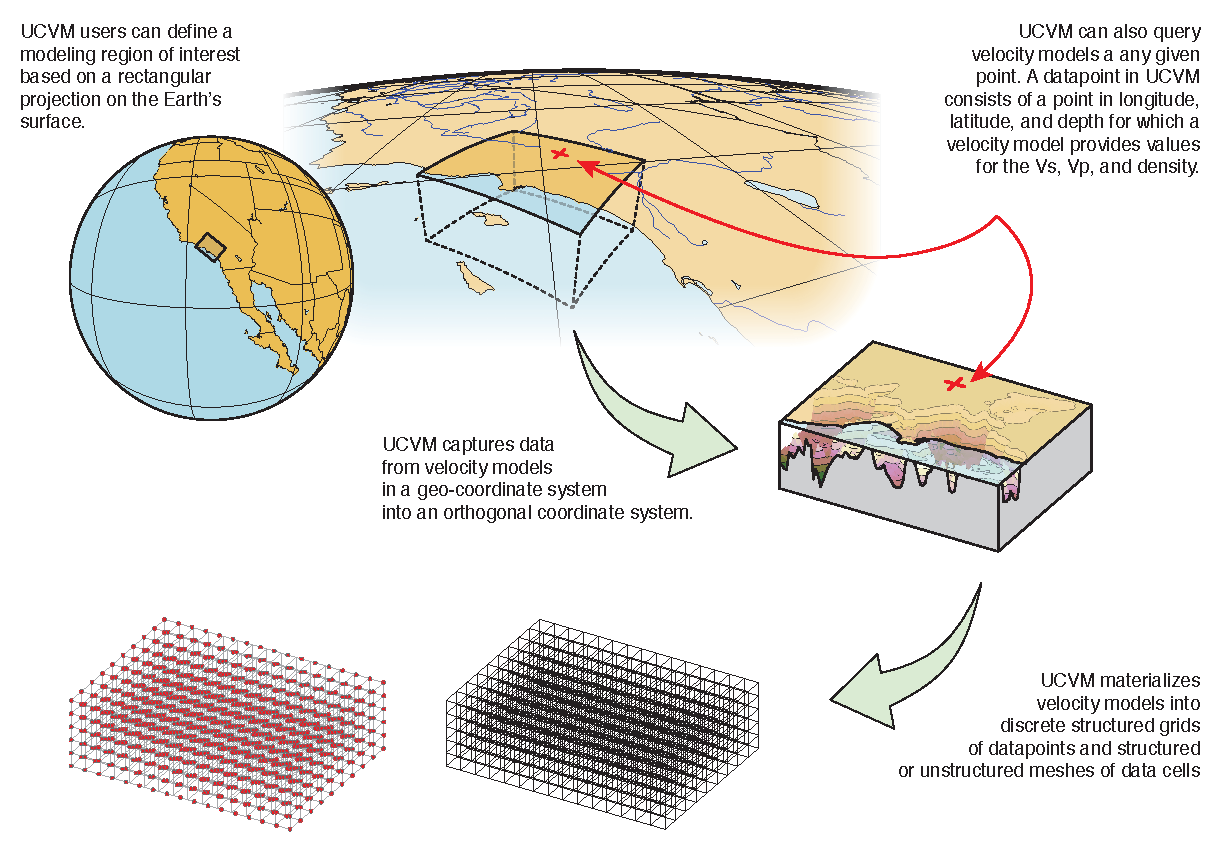
\includegraphics
		[width=0.85\textwidth]
		{figures/pdf/ucvm-model-extraction}
	\caption{High-level description of the UCVM framework functionality illustrating the selection of a region of interest for which a user can obtain datapoints using the UCVM utilities and create materialized models in the form of discrete three-dimensional grids or meshes.}
	\label{fig:framework}
\end{figure*}




\begin{figure*}[ht!]
	\centering
	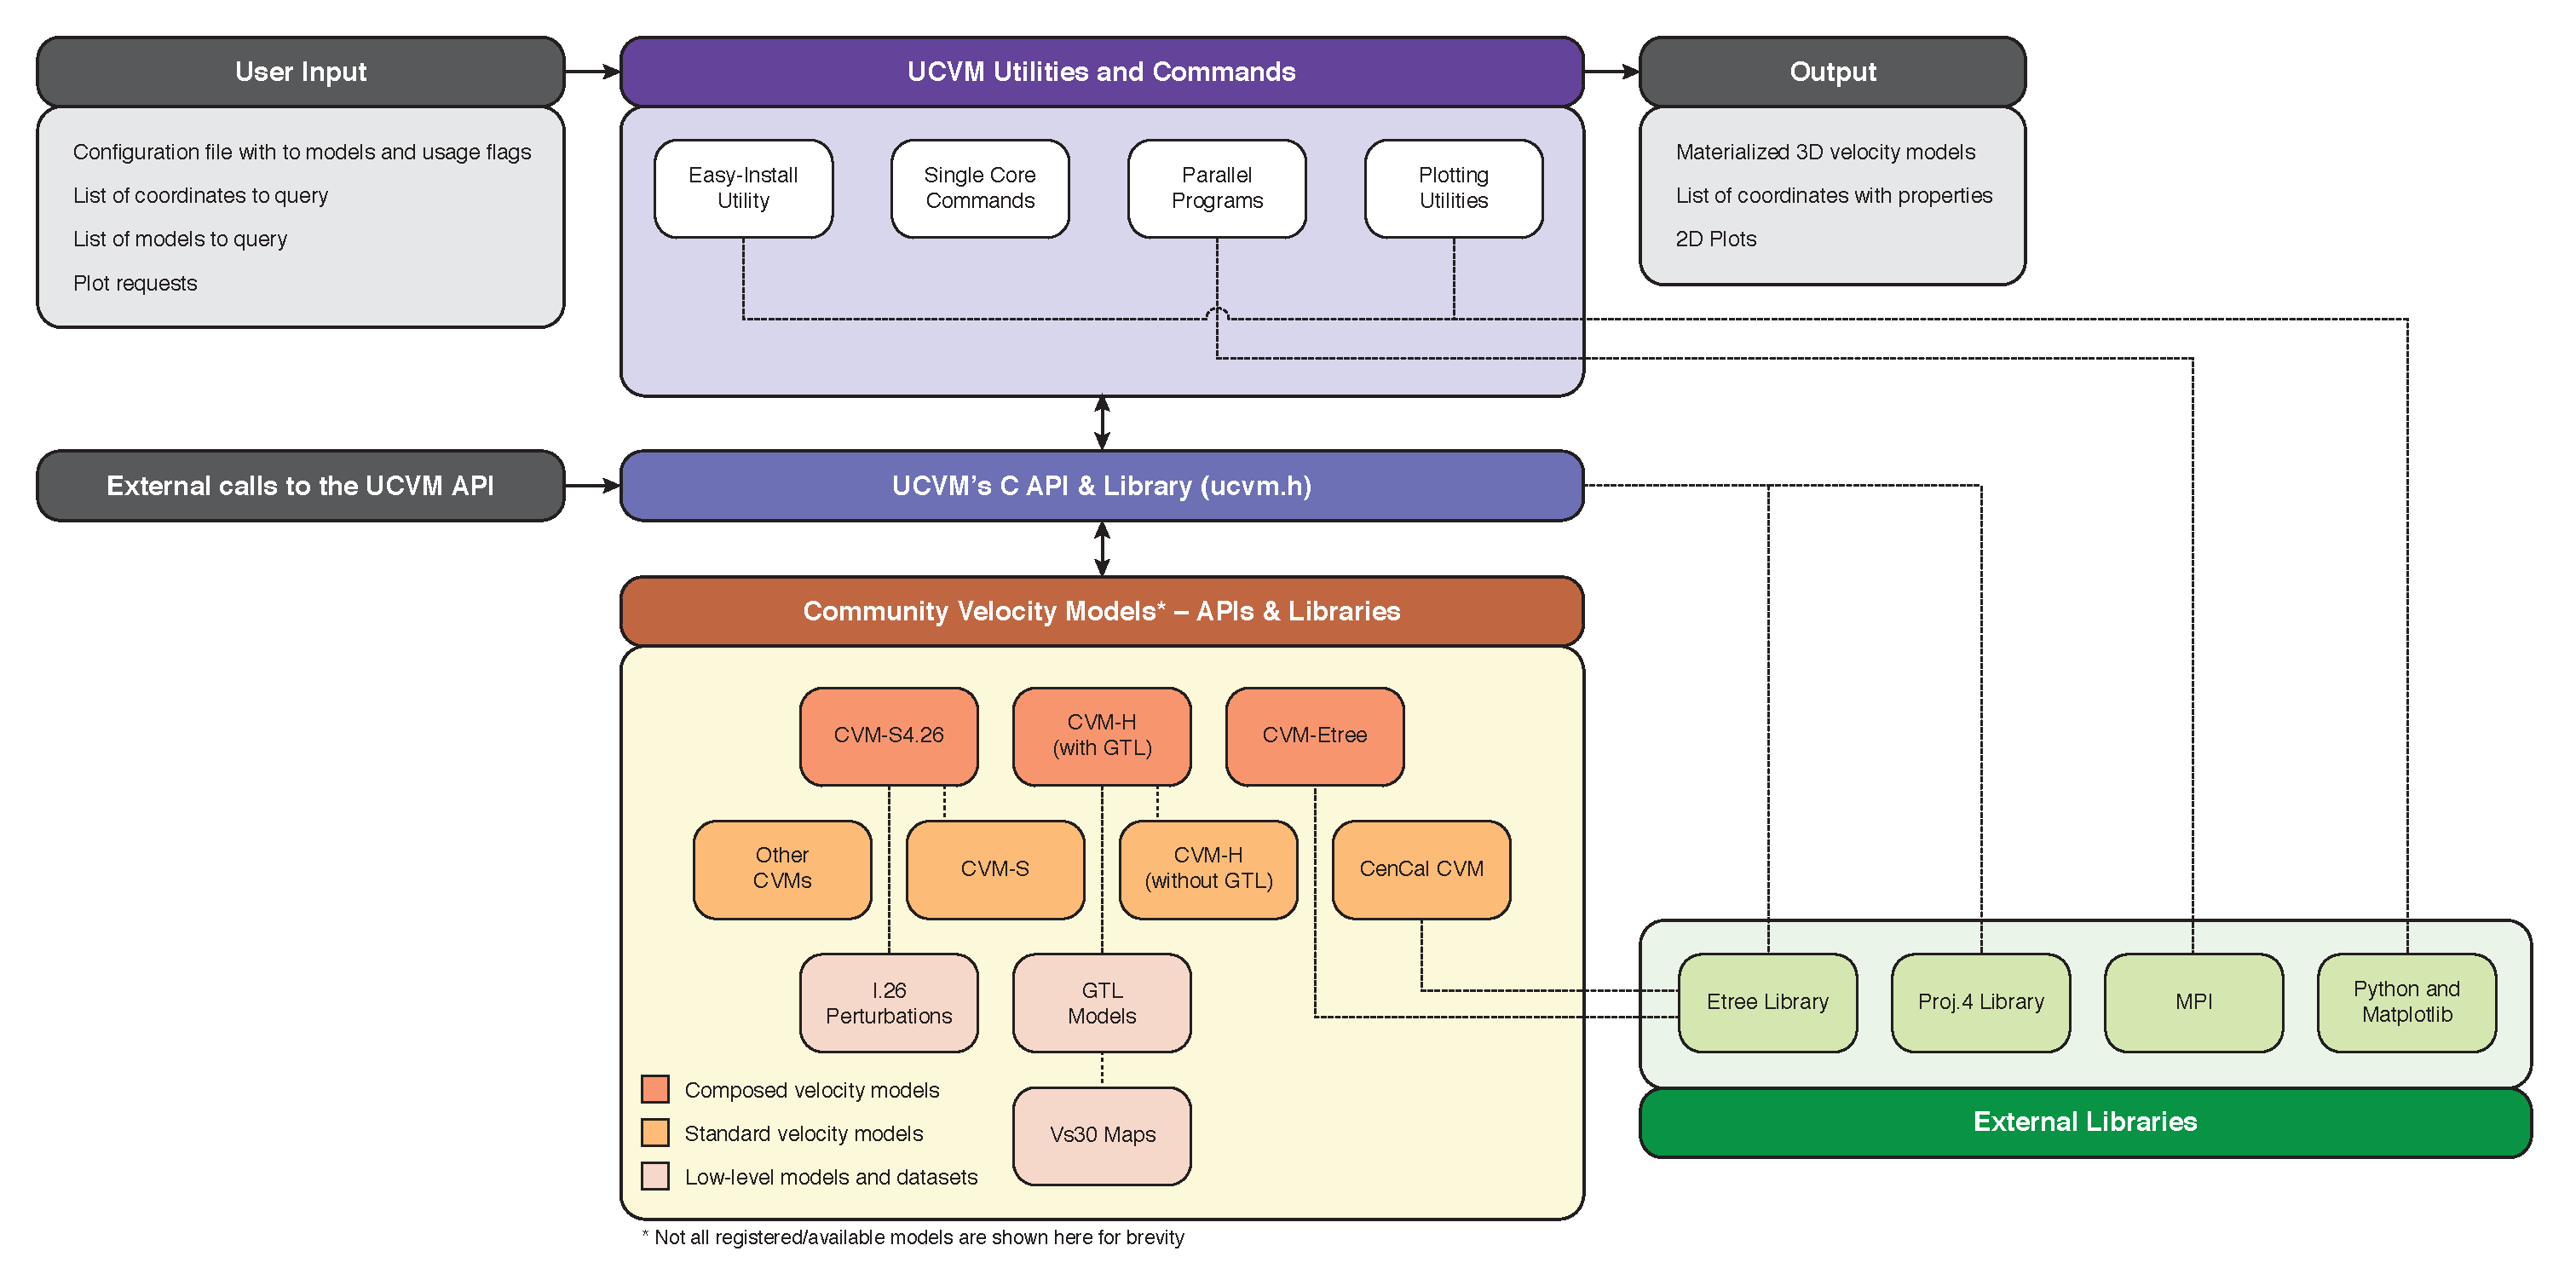
\includegraphics
		[width=\textwidth]
		{figures/pdf/ucvm-sw-architecture}
	\caption{The UCVM software architecture. Gray-colored frames indicate components at the level of user or client interaction. The upper purple-colored frame displays UCVM utilities and commands directly accessible to users, whereas the ligher purpled-colored box indicates the lower-level UCVM API and library upon which UCVM operations rest. Underlying this, are a selection of community models supported by UCVM; and to the right, in green, are the library dependencies of the UCVM framework. Here we distinguish models and datasets in four categories related to their origin or operational concept. In practice, however, UCVM treats each model or dataset independently and without any distinction.}
	\label{fig:sw.arch}
\end{figure*}



\begin{table*}
\centering
\small
\caption{Electronic addresses to UCVM on-line documentation.}
\begin{tabular}[]{ll}
\\
Description                 & URL Address                                                         \\
\hline
General Documentation       & \url{http://scec.usc.edu/scecpedia/UCVM}                            \\
General User Guide          & \url{http://scec.usc.edu/scecpedia/UCVM_User_Guide}                 \\
Latest Version (14.3) Guide & \url{http://scec.usc.edu/scecpedia/UCVM_14.3.0_User_Guide}          \\
Advanced User Guide (14.3)  & \url{http://scec.usc.edu/scecpedia/UCVM_14.3.0_Advanced_User_Guide} \\
Tutorial (14.3)             & \url{http://scec.usc.edu/scecpedia/UCVM_14.3.0_Tutorial}            \\
\hline
\end{tabular}
\label{tab:manuals}
\end{table*}


\section{The UCVM Software Framework}\label{sec:ucvm}

\subsection{Overview}

The primary functionality provided by UCVM is the ability to query a wide array of CVMs for material properties through a standardized query interface, and return material properties from the CVMs in standardized formats, independently of the particularities of each dataset or CVM. UCVM achieves this by registering datasets and velocity models into the framework. Registration of a velocity model or dataset consists of creating the appropriate API to facilitate the communication between the framework utilities and tools, and the velocity models and datasets. Once a velocity model or dataset has been registered with UCVM, a client can use the framework utilities to retrieve information from the models at any geographic point within the coverage region of the model(s). A client can be either a user (via the command-line) or a software application. The primary data type retrieved by a UCVM client for a single geographical point consists of a float triplet with the seismic velocities (\vp{} and \vs{}), and the material's density ($\rho$). At times we refer to this triple as the payload. The UCVM can then be used to produce standardized output in the form of three-dimensional (3D) volumetric datasets, two-dimensional (2D) vertical cross-sections and horizontal slices, and individual data points. This process is illustrated at a general level for the cases of 3D models in Figure \ref{fig:framework}. A client can also use other UCVM utilities for plotting and transforming models and datasets.

In order to facilitate access to the models, UCVM conceals each model's local coordinate system behind a generic querying interface. Data points are queried through this interface by geographic latitude and longitude, and a vertical $z$-coordinate. The framework allows defining the $z$-axis as either depth below the free surface (in meters, positive downward) or elevation relative to mean sea level (where zero is at sea level, positive upward and negative downward). The UCVM standardized interface allows multiple velocity models to be aggregated into a single composite model or meta-model. Composition is accomplished by tiling two or more velocity models in three dimensions according to a user-specified priority order. To support this flexible query mechanism consistently across all models, UCVM includes a high-resolution digital elevation model (DEM) and uses a cartographic projection library (Proj.4: \url{http://trac.osgeo.org/proj}). The DEM is synthesized from the U.S.~Geological Survey (USGS) National Elevation Dataset \citep{Gesch_2002_PERS, Gesch_2007_Chap} and the ETOPO1 Global Relief Model \citep{Amante_2009_Manual}. The built-in DEM enables clients to retrieve the surface elevation at any query point in addition to the default data-point payload of material properties (\vp{}, \vs{}, $\rho$).

The abstraction of native CVM interfaces under a uniform API is illustrated by Figure \ref{fig:sw.arch}. This API is written in the C language, and may be invoked directly by an application program to query any registered model as described previously. Alternatively, the framework provides a small set of predefined command-line tools to perform common operations, such as querying points, creating meshes, and producing simple graphs. As these tools are themselves defined in terms of the API, they may be leveraged as templates for creating new utilities. This layered approach to the framework design allows for future extensibility both in terms of new model support, and querying functionality.

With the exception of the Wasatch Front (Utah) CVM, the primary focus area of UCVM has been on models available for the State of California (and portions of neighboring States). However, the framework has been designed to be easily modified to cover any arbitrary region of the Earth's surface, provided adequate resolution velocity and elevation models exist. Additional details about the models available through UCVM are given in the following section on Community Velocity Models. Subsequent sections provide further information on the main UCVM features. However, due to space limitations, not all utilities and options are described in detail here. For additional in-depth information, general and advanced users should refer to the on-line manuals and documentation. Table \ref{tab:manuals} provides URL addresses linking to permanent supporting material. The last section of the paper is dedicated to simple examples and recent case applications of UCVM. 



\begin{figure*}[ht!]
	\centering
	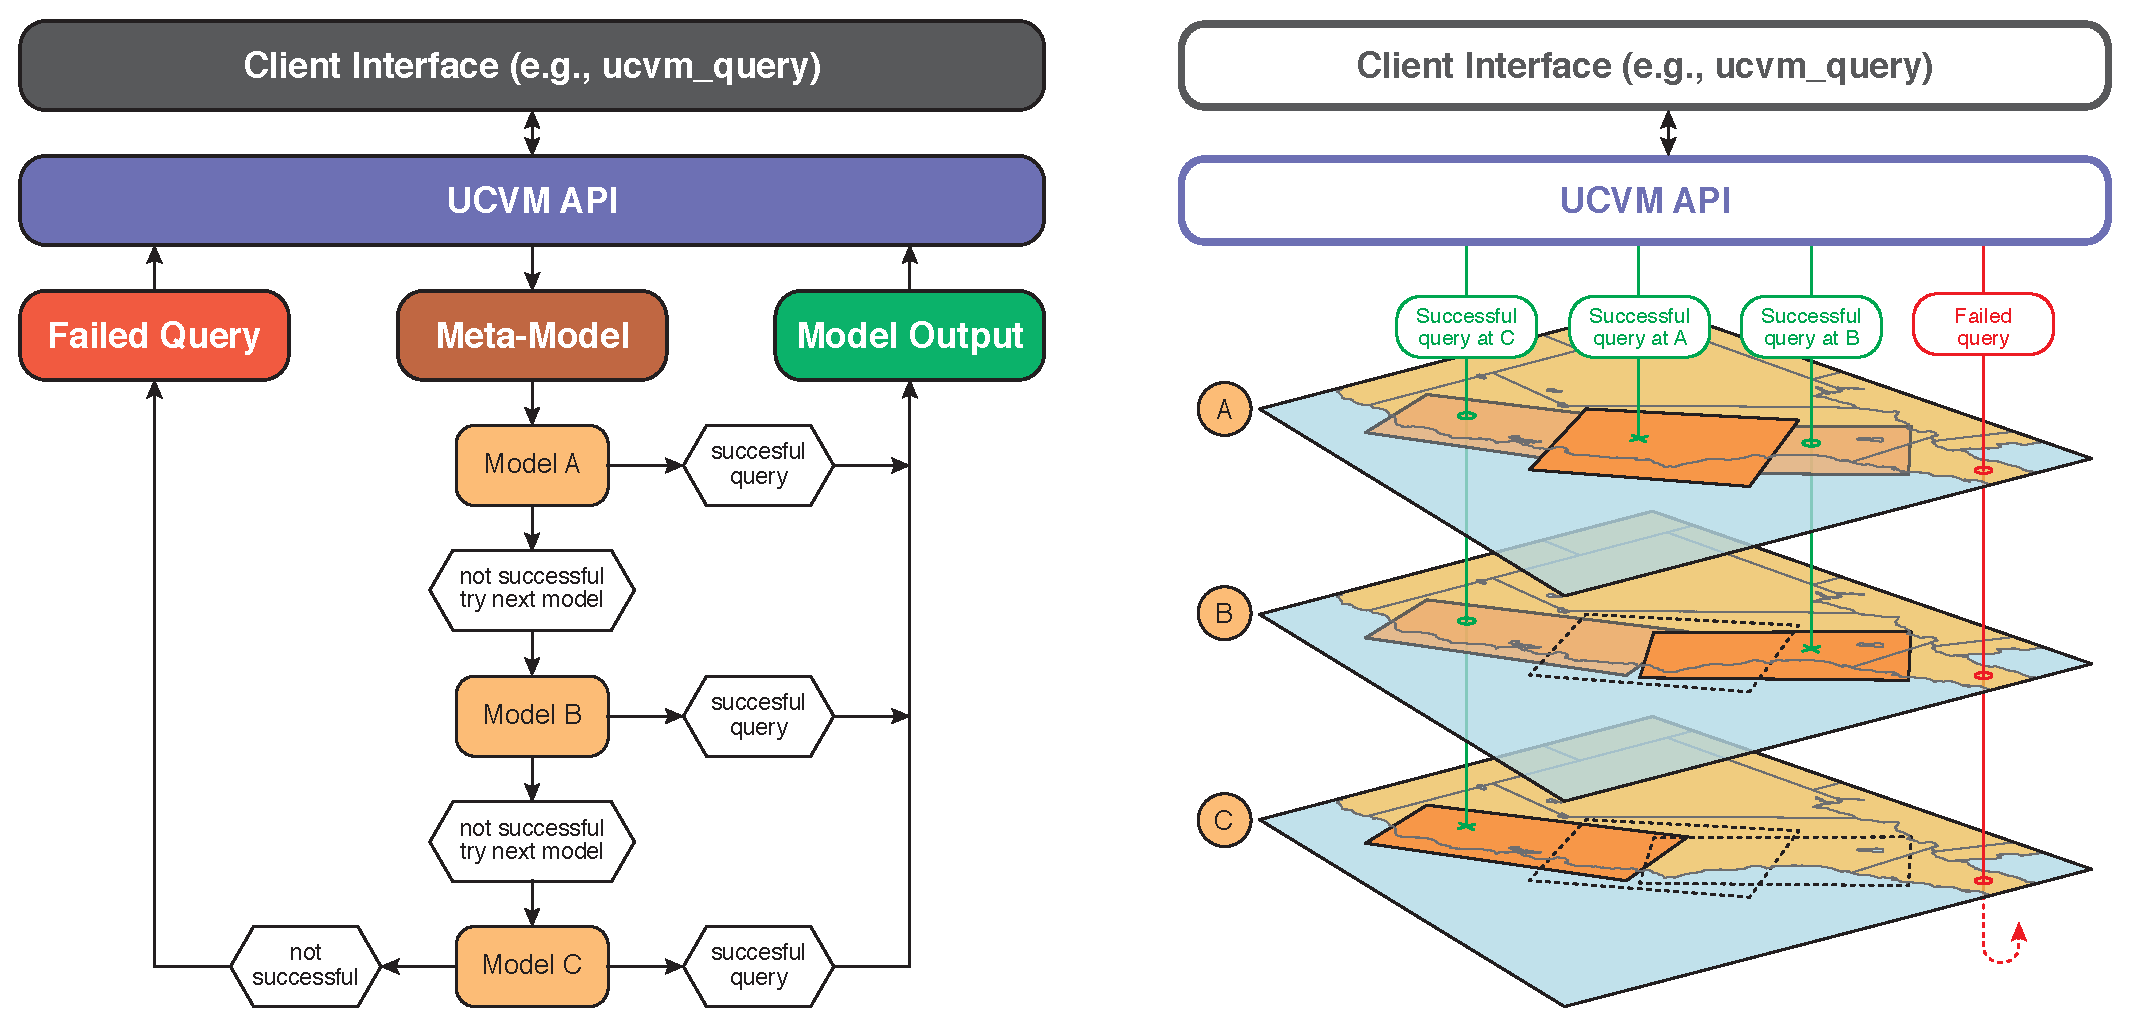
\includegraphics
		[width=0.75\textwidth]
		{figures/pdf/ucvm-query}
	\caption{UCVM querying scheme (left) and geographical illustration of the querying process (right). Information at a given geographic location is retrieved from the models registered in UCVM through a hierarchical querying scheme in which the user defines a preferred sequence of models, which are assembled internally in a meta-model. Queries to the models beneath the meta-model are carried out in the order specified by the user. Successful queried values (or failed-query results) are handled by the UCVM API wich is accessible to the user/client through a predefined interface such as the program \texttt{ucvm\_query}.}
	\label{fig:tiling}
\end{figure*}


\subsection{Querying Material Properties}
\label{sec:querying}

UCVM provides two methods for querying models. The first method is programmatically, directly through the provided C language API. The second is via the command-line program \texttt{ucvm\_query}. Both methods query the underlying models in the same manner; the \texttt{ucvm\_query} program is merely a simplified front-end layered upon the API.

The query process begins with the identification of one or more CVMs as the source of material properties. In this respect, the framework distinguishes between geotechnical layers and standard crustal models, allowing the user to make selections for both. As illustrated in Figure \ref{fig:tiling}, the set of standard crustal models is tiled in three dimensions to form a meta-model. The same operation is performed on the GTLs to define a meta-GTL. The interface between the meta-GTL and meta-model is then smoothed using an interpolation function (linear interpolation in the simplest case) along a user-defined interpolation zone parallel to the z-axis. Note that when two or more models overlap in three dimensional space, the model listed first within the tiling order will satisfy requests within that overlapping zone.

Once the models have been tiled in this manner, the API or program accepts one or more input query points from the user. For every point, the framework queries each component model of the two meta models, until either a valid set of velocities and density are returned, or all component models have been queried and the request was unsatisfied. Thus, for points that fall within the interpolation zone, two sets of material properties may be generated---one for each meta model. These two sets of material properties are then combined using the interpolation function. As the native query interfaces of available CVMs accept query points in a wide array of formats (e.g., geographic coordinates versus UTM-11 map coordinates, or depth versus elevation for the vertical component), UCVM may perform a coordinate transformation to convert its input format of decimal (latitude, longitude, depth/elevation) tuples to the local coordinate system of the component model being queried. This is accomplished transparently by utilizing the standard projection library Proj.4 \citep{Evenden_2003_Manual}.

In the case of the API, the result of a successful query is a data-structure containing the velocities \vp{} and \vs{}, and the density $\rho$ at the point of interest, along with the elevation in meters and $V_{S30}$ value of the corresponding point on the free-surface. This data-structure also includes an indicator of which velocity model within the meta-model ultimately satisfied the request. For those points which fall within the interpolation zone between the meta-GTL and meta-model, the framework additionally identifies the material properties reported by the meta-GTL and the meta-model, as well as the component models from which they were extracted. For the \texttt{ucvm\_query} program, this same information is formulated in tabular format and printed to the screen.

This tiling mechanism mostly allows one to complement missing information in one model with that of other overlapping or underlying models. In the future, the UCVM tiling feature could be used as tool for combining multiple regional velocity models. The platform, however, does not presently provide built-in functionalities to do so beyond the described tiling mechanism. The reason being that consistency problems arise when velocity models overlap in three-dimensional space. That is, tiling two overlapping models that are not compatible has the potential of creating interfaces with unnatural contrasts. These artifacts are undesirable for earthquake simulation applications because they can cause unexpected wave reflections or refractions. There are two approaches one can take to remedy this problem. The simplest approach is to define a UCVM patch model to trilinearly interpolate the material properties within a certain geographic region. This patch model may be tiled along with the overlapping traditional velocity models to produce a smoothed meta-model. However, this numerical smoothing approach may not reflect the physical structures of the Earth's surface. The second approach is to utilize UCVM to query all models within the overlap zone individually, and then manually combine the results with a user-defined interpolation function. We expect that future tomographic inversions of larger regions will allow us to integrate better models or algorithms to handle this situation.


\section{Community Velocity Models}
\label{sec:cvms}

The UCVM framework supports different seismic velocity models. 

(temp material)

Community velocity models vary widely in their area of coverage, depth extent, and resolution. UCVM is flexible in its support for such variability. However, in order to better accommodate high frequency ground motion simulations, it categorizes models into two general groups: crustal models, and geotechnical layers (GTLs). Crustal models provide subsurface seismic wave velocities associated with basin, crust, and mantle structures. These models may potentially extend to many tens of kilometers below the Earth's surface yet do so at coarse resolutions (TODO: cite CVM-H, CVM-S). Geotechical layers, in contrast, provide velocities for only the near-surface (typically a few hundred meters) at very high resolution (TODO: cite Ely Vs30 GTL). Ground motion simulations, in particular, rely on high-resolution near-surface velocities and therefore a GTL serves to supplement the coarser data provided by crustal models.

TODO: Interpolation of GTL with Crustal

%\textit{
%\color{blue}
%This section will present how CVMs work and the various CVMs available to the community today. It will basically explain that CVMs provide the triplets of Vs, Vp and density, and, as an example, we can expand on a description of CVM-S and CVM-H, including their variations CVM-SI and CVM-H+GTL.
%}


